%  _____________________________________
%
%   Trabalho Acadêmico (LaTeX template)
%  _____________________________________
%  
%  * Universidade de Pernambuco 
%  * Por Thiago Ribeiro. 		
%
%  Fique à vontade para modificar o documento e deixe ao 
%  seu gosto. Bom proveito! :)

\documentclass[12pt]{article}
\usepackage[misc]{ifsym}
% Pacotes para expressões matemáticas
\usepackage{amsmath}
\usepackage{MnSymbol}
\usepackage{wasysym}
% Ajuste de margens
\usepackage[top=2.5cm, left=3cm, right=3cm, bottom=2cm, headheight=110pt]{geometry} 
\usepackage[brazilian]{babel}
\usepackage[utf8]{inputenc}\usepackage[T1]{fontenc}
\usepackage{graphicx}
\usepackage{color, colortbl}
% Header
\usepackage{fancyhdr}
\pagestyle{fancy}
\usepackage{cite}

\linespread{1.27} % espaçamento entre linhas 

% Início do documento
\begin{document}
	\thispagestyle{empty}
	\begin{figure}[!htp]
	    {
\includegraphics[scale=0.2, width=2.4cm]{../imagens/poli.png}}\hfill%
	    {
\includegraphics[scale=0.3, width=3.7cm]{../imagens/ecomp.png}}%
  	\end{figure}
	\vspace{3.5cm}

	\begin{center}
		% \PaperPortrait % Substituir por outro ícone caso queira		
		\Large{ \ {\bf Título do Documento}}\\[0.2cm]
		\large{Sub-título do Documento}
	\end{center}
	
	\vspace{5cm}
	\begin{center}
		\begin{tabular}{rl}
			{\bf Disciplina:} & {\sf COMP01 - Nome da Disciplina}\\
			{\bf Professor:} & {\sf Nome do professor}\\
			{\bf Aluno:} & {\sf Nome do aluno}\\
			{\bf Outro:} & {\sf Conteúdo adicional}\\
		\end{tabular}
	\end{center}
	\vspace{3.5cm}
	\begin{center}
		{\sc mês ano}\\{\sc Outra informação}\\
	\end{center}
	\newpage

	\tableofcontents
	
	\newpage
	
	\section{Introdução}
	\subsection{Objetivo}
	
	Give me a flammable life, I'm cold as a match ready to strike so here I go Here lies a city on fire singing along the arsonist choir now here I go it started with a spark and burned into the dark now here I go, there's a river I've found into the wild, under the ground so here I go.
	
	\begin{figure}[!htb]
	    \centering
	    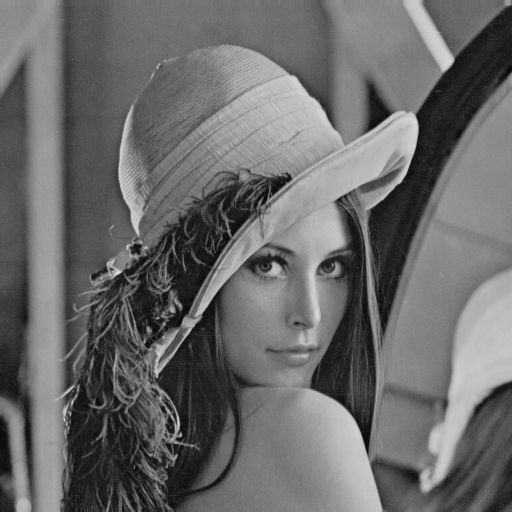
\includegraphics[scale=0.3]{../imagens/lena.jpg}
	    \caption{Título da imagem.}
	    \label{fig:lena}
	\end{figure}
	
	You can also add equations like this:

	\begin{equation} \label{eq1}
		\begin{split}
		A & = \frac{\pi r^2}{2} \\
		 & = \frac{1}{2} \pi r^2
		\end{split}
	\end{equation}

	\subsection{Escopo do Projeto}
	
	Oh sweet ignition, be my fuse you had no choice you have to choose, bid farewell to yesterday, say goodbye I'm on my way.

	\begin{itemize}
		\item Descrição do item:
		\begin{itemize}
			\item {\it Sub-item 1};
			\item {\it Sub-item 2};
			\item {\it Sub-item 3;}
		\end{itemize}
	\end{itemize}
	
	\section{Título}
	\subsection{Sub-título}

	A million miles away your signal in the distance to whom it may concern I think I lost my way getting good at starting over everytime that I return.

	\section{Referências}
	
	Why won't you let me twist your faith it's getting kinda late but I don't wanna wait no more well may I have this dance of day locked in your embrace passed your test of faith\cite{ahu61}

	\bibliographystyle{ieeetr}

	\bibliography{research}{}
	
\end{document}